\section{Orações Complementares}

\subsection{Acção de Graças da Missa}

\begin{paracol}{2}\latim{
\emph{Ant.} Trium puerórum cantémus hymnum, quem cantábant Sancti in camíno ignis, benedicéntes Dóminum. (T. P. Allelúja.)
}\switchcolumn\portugues{
\emph{Ant.} Cantemos o hino dos três jovens que cantavam os Santos na fornalha do fogo, glorificando o Senhor. (T. P. Aleluia.)
}\end{paracol}

\subsubsection{Benedícite}
\begin{paracol}{2}\latim{
\rlettrine{B}{enedícite,} ómnia ópera Dómini, Dómino: laudáte et superexaltáte eum in sǽcula.
}\switchcolumn\portugues{
\rlettrine{B}{endizei} o Senhor, todas as obras do Senhor; louvai-O e aclamai-O em todos os séculos.
}\switchcolumn*\latim{
Benedícite, Angeli Dómini, Dómino: benedícite, cœli, Dómino.
}\switchcolumn\portugues{
Anjos do Senhor, bendizei o Senhor; céus, bendizei o Senhor.
}\switchcolumn*\latim{
Benedícite, aquæ omnes, quæ super cœlos sunt, Dómino: benedícite, omnes virtútes Dómini, Dómino.
}\switchcolumn\portugues{
Águas todas, que estai nos espaços celestiais, bendizei o Senhor; bendizei o Senhor, todos os exércitos do Senhor.
}\switchcolumn*\latim{
Benedícite, sol et luna, Dómino: benedícite, stellæ cœli, Dómino.
}\switchcolumn\portugues{
Bendizei o Senhor, sol e lua; bendizei o Senhor, estrelas do céu.
}\switchcolumn*\latim{
Benedícite, omnis imber et ros, Dómino: benedícite, omnes spíritum Dei, Dómino.
}\switchcolumn\portugues{
Chuvas e orvalhos, bendizei todos o Senhor; ventos, bendizei todos o Senhor.
}\switchcolumn*\latim{
Benedícite, ignis et æstus, Dómino: benedícite, frigus et æstus. Dómino.
}\switchcolumn\portugues{
Bendizei o Senhor, ó fogo e chamas; bendizei o Senhor, ó frio e frio gélido.
}\switchcolumn*\latim{
Benedícite, rores et pruína, Dómino: benedícite, gelu et frigus, Dómino.
}\switchcolumn\portugues{
Ó orvalhos e chuvas, bendizei o Senhor; ó neves e gelos, bendizei o Senhor.
}\switchcolumn*\latim{
Benedícite, glácies et nives, Dómino: benedícite, noctes et dies, Dómino:
}\switchcolumn\portugues{
Bendizei o Senhor, ó granizos e geadas; bendizei o Senhor, ó noites e dias.
}\switchcolumn*\latim{
Benedícite, lux et ténebræ, Dómino: benedícite, fúlgura et nubes, Dómino.
}\switchcolumn\portugues{
Luz e trevas, bendizei o Senhor; relâmpagos e tempestades, bendizei o Senhor.
}\switchcolumn*\latim{
Benedícat terra Dóminum: laudet et superexáltet eum in sǽcula.
}\switchcolumn\portugues{
Que a terra bendiga o Senhor; que O louve e aclame em todos os séculos.
}\switchcolumn*\latim{
Benedícite, montes et colles, Dómino: benedícite, univérsa germinántia in terra, Dómino.
}\switchcolumn\portugues{
Ó montes e colinas, bendizei o Senhor; ó todos os seres, que germinais na terra, bendizei o Senhor.
}\switchcolumn*\latim{
Benedícite, fontes, Dómino: benedícite, mária et flúmina, Dómino.
}\switchcolumn\portugues{
Bendizei o Senhor, ó fontes; bendizei o Senhor, ó mares e rios.
}\switchcolumn*\latim{
Benedícite, cete, et ómnia, quæ movéntur in aquis, Dómino: benedícite, omnes vólucres cœli, Dómino.
}\switchcolumn\portugues{
Peixes e todos os entes, que vos moveis nas águas, bendizei o Senhor; aves do céu, bendizei todas o Senhor.
}\switchcolumn*\latim{
Benedícite, omnes béstiæ et pécora, Dómino: benedícite, fílii hóminum, Dómino.
}\switchcolumn\portugues{
Ó animais e rebanhos, bendizei todos o Senhor, bendizei o Senhor, ó filhos dos homens.
}\switchcolumn*\latim{
Benedícat Israël Dóminum: laudet et superexáltet eum in sǽcula.
}\switchcolumn\portugues{
Bendizei o Senhor, ó Israel: louvai-O e aclamai-O em todos os séculos.
}\switchcolumn*\latim{
Benedícite, sacerdótes Dómini, Dómino: benedícite, servi Dómini, Dómino.
}\switchcolumn\portugues{
Sacerdotes do Senhor, bendizei o Senhor; servos do Senhor, bendizei o Senhor.
}\switchcolumn*\latim{
Benedícite, spíritus, et ánimæ justórum, Dómino: benedÌcite, sancti, et húmiles corde, Dómino.
}\switchcolumn\portugues{
Bendizei o Senhor, ó espíritos e almas dos justos; bendizei o Senhor, ó santos e humildes de coração.
}\switchcolumn*\latim{
Benedícite, Ananía, Azaría, Mísaël, Dómino: laudáte et superexaltáte eum in sǽcula.
}\switchcolumn\portugues{
Bendizei o Senhor, ó Ananias, Azarias e Misael: louvai-O e exaltai-O em todos os séculos.
}\switchcolumn*\latim{
Benedicámus Patrem et Filium cum Sancto Spíritu: laudémus et superexaltémus eum in sǽcula.
}\switchcolumn\portugues{
Bendigamos o Pai, e o Filho, assim como o Espírito Santo: louvemo-l’O e aclamemo-l’O em todos os séculos.
}\switchcolumn*\latim{
Benedíctus es, Dómine, in firmaménto cœli: et laudábilis, et gloriósus, et superexaltátus in sǽcula.
}\switchcolumn\portugues{
Bendito sois, Senhor, no firmamento do céu, e digno de ser louvado e aclamado em todos os séculos.
}\end{paracol}


\subsubsection{Salmo 150}
\begin{paracol}{2}\latim{
\rlettrine{L}{audáte} Dóminum in sanctis ejus: * laudáte eum in firmaménto virtútis ejus.
}\switchcolumn\portugues{
\rlettrine{L}{ouvai} o Senhor no seu santuário: * louvai-O no seu augusto firmamento.
}\switchcolumn*\latim{
Laudáte eum in virtútibus ejus: * laudáte eum secúndum multitúdinem magnitúdinis ejus.
}\switchcolumn\portugues{
Louvai-O nas suas virtudes: * louvai-O segundo a multidão da sua grandeza.
}\switchcolumn*\latim{
Laudáte eum in sono tubæ: * laudáte eum in psaltério, et cíthara.
}\switchcolumn\portugues{
Louvai-O ao som da trombeta: * louvai-O com o saltério e a cítara.
}\switchcolumn*\latim{
Laudáte eum in týmpano, et choro: * laudáte eum in chordis, et órgano.
}\switchcolumn\portugues{
Louvai-O com timbales e em coro: * louvai-O com cordas e órgão.
}\switchcolumn*\latim{
Laudáte eum in cýmbalis benesonántibus: laudáte eum in cýmbalis jubilatiónis: * omnis spíritus laudet Dóminum.
}\switchcolumn\portugues{
Louvai-O com címbalos melodiosos: louvai-O com címbalos de júbilo: * todo o espirito louve o Senhor.
}\end{paracol}


\begin{paracol}{2}\latim{
\emph{Ant.} Trium puerórum cantémus hymnum, quem cantábant Sancti in camíno ignis, benedicéntes Dóminum. (T. P. Allelúja.)
}\switchcolumn\portugues{
\emph{Ant.} Cantemos o hino dos três jovens que cantavam os Santos na fornalha do fogo, glorificando o Senhor. (T. P. Aleluia.)
}\switchcolumn*\latim{
Kýrie, eléison. Christe, eléison. Kýrie, eléison.
}\switchcolumn\portugues{
Senhor, tende piedade de nós. Cristo, tende... Senhor, tende...
}\switchcolumn*\latim{
Pater noster. ℣. Et ne nos indúcas in tentatiónem. ℞. Sed líbera nos a malo.
}\switchcolumn\portugues{
Pai-nosso. ℣. E não nos deixeis cair em tentação. ℟. Mas livrai-nos do mal.
}\switchcolumn*\latim{
℣. Confiteántur tibi, Dómine, omnia opera tua. ℞. Et Sancti tui benedícant tibi.
}\switchcolumn\portugues{
℣. Que todas vossas obras Vos louvem, Senhor. ℟. E os vossos Santos Vos bendigam.
}\switchcolumn*\latim{
℣. Exsultábunt Sancti in glória. ℞. Lætabúntur in cubílibus suis.
}\switchcolumn\portugues{
℣. Os Santos exultam de alegria. ℟. Alegrar-se-ão no lugar do seu repouso.
}\switchcolumn*\latim{
℣. Non nobis, Dómine, non nobis. ℞. Sed nómini tuo da glóriam.
}\switchcolumn\portugues{
℣. Não a nós, Senhor, não a nós. ℟. Mas ao vosso nome dêmos glória.
}\switchcolumn*\latim{
℣. Dómine, exáudi oratiónem meam. ℞. Et clamor meus ad te véniat.
}\switchcolumn\portugues{
℣. Senhor, ouvi a minha oração. ℟. E o meu clamor chegue até Vós.
}\switchcolumn*\latim{
℣. Dóminus vobíscum.
}\switchcolumn\portugues{
℣. O Senhor seja convosco.
}\switchcolumn*\latim{
℞. Et cum spíritu tuo.
}\switchcolumn\portugues{
℟. E com vosso espírito.
}\switchcolumn*\latim{
\begin{nscenter} Orémus. \end{nscenter}
}\switchcolumn\portugues{
\begin{nscenter} Oremos. \end{nscenter}
}\switchcolumn*\latim{
\rlettrine{D}{eus,} qui tribus púeris mitigásti flammas ígnium: concéde propítius; ut nos fámulos tuos non exúrat flamma vitiórum.
}\switchcolumn\portugues{
\slettrine{Ó}{} Deus, que mitigastes aos três jovens as chamas da fornalha ardente, concedei-nos benigno que nós, vossos servos, não sejamos consumidos pelas chamas dos vícios.
}\switchcolumn*\latim{
\rlettrine{A}{ctiónes} nostras, quǽsumus, Dómine, aspirándo prǽveni et adjuvándo proséquere: ut cuncta nostra orátio et operátio a te semper incípiat, et per te cœpta finiátur.
}\switchcolumn\portugues{
\rlettrine{D}{ignai-Vos,} Senhor, insuflar as nossas acções com vosso espírito e acompanhá-las com vossa graça, a fim de que todas nossas orações e obras, tendo princípio em Deus, tenham nele a finalidade.
}\switchcolumn*\latim{
\rlettrine{D}{a} nobis, quǽsumus, Dómine, vitiórum nostrórum flammas exstínguere: qui beáto Lauréntio tribuísti tormentórum suórum incéndia superáre. Per Christum, Dóminum nostrum. ℞. Amen.
}\switchcolumn\portugues{
\rlettrine{S}{enhor,} assim como concedestes ao bem-aventurado Lourenço a fortaleza para vencer o tormento do fogo, assim também, Vos suplicamos, dignai-Vos permitir que extingamos as chamas dos nossos vícios. Por Cristo, nosso Senhor.
℟. Amen.
}\end{paracol}

\subsubsection{Oração São Tomás Aquino}

\begin{paracol}{2}\latim{
\rlettrine{G}{rátias} tibi ago, Dómine sancte, Pater omnípotens, ætérne Deus, qui me peccatórem, indígnum fámulum tuum, nullis meis méritis, sed sola dignatióne misericórdiæ tuæ satiáre dignátus es pretióso Córpore et Sánguine Filii tui. Dómini nostri Jesu Christi. Et precor, ut hæc sancta commúnio non sit mihi reátus ad pœnam, sed intercéssio salutáris ad véniam. Sit mihi armatúra fídei et scutum bonæ voluntátis. Sit vitiórum meórum evacuátio, concupiscéntiæ et libídinis exterminátio, caritátis et patiéntiæ, humilitátis et obœdiéntiæ, omniúmque virtútum augmentátio: contra insídias inimicórum ómnium, tam visibílium quam invisibílium, firma defénsio: mótuum meórum, tam carnálium quam spiritálium, perfécta quietátio: in te uno ac vero Deo firma adhǽsio; atque finis mei felix consummátio. Et precor te, ut ad illud ineffábile convívium me peccatórem perdúcere dignéris, ubi tu cum Fílio tuo et Spíritu Sancto Sanctis tuis es lux vera, satíetas plena, gáudium sempitérnum, jucúnditas consummáta et felícitas perfécta. Per eúndem Christum, Dóminum nostrum. Amen.
}\switchcolumn\portugues{
\rlettrine{D}{ou-Vos} graças, Senhor santo, Pai omnipotente, Deus eterno, a Vós que, sem merecimento nenhum da minha parte, mas por efeito de vossa misericórdia, Vos dignastes saciar-me, sendo eu pecador e vosso indigno servo, com o Corpo adorável e com o Sangue precioso do vosso Filho, Nosso Senhor Jesus Cristo. Eu Vos peço que me não seja esta comunhão imputada como uma falta digna de castigo, mas interceda eficazmente para alcançar o meu perdão; seja a armadura da minha fé e o escudo da minha boa vontade; livre-me dos meus vícios; apague os meus maus desejos; mortifique a minha concupiscência; aumente em mim a caridade e a paciência, a humildade, a obediência e todas as virtudes; sirva-me de firme defesa contra os embustes de todos meus inimigos, tanto visíveis como invisíveis; serene e regule perfeitamente todos os movimentos, tanto da minha carne como do meu espírito; una-me firmemente a Vós, que sois o único e verdadeiro Deus; e seja, enfim, a feliz consumação do meu destino. Dignai-Vos, Senhor, eu Vos suplico, conduzir-me, a mim pecador, a esse inefável festim, onde, com vosso Filho e o Espírito Santo, sois para os vossos santos luz verdadeira, gozo pleno e alegria eterna, cúmulo de delícias e felicidade perfeita. Pelo mesmo N. S. Jesus Cristo. Amen.
}\end{paracol}

\subsubsection{Oração São Boaventura}

\begin{paracol}{2}\latim{
\rlettrine{T}{ransfíge,} dulcíssime Dómine Jesu, medúllas et víscera ánimæ meæ suavíssimo ac salubérrimo amóris tui vúlnere, vera serenáque et apostólica sanctíssima caritáte, ut lángueat et liquefíat ánima mea solo semper amóre et desidério tui; te concupíscat et defíciat in átria tua, cúpiat dissólvi et esse tecum. Da, ut ánima mea te esúriat, panem Angelórum, refectiónem animárum sanctárum, panem nostrum cotidiánum, supersubstantiálem, habéntem omnem dulcédinem et sapórem et omne delectaméntum suavitátis. Te, in quem desíderant Angeli prospícere, semper esúriat et comédat cor meum, et dulcédine sapóris tui repleántur víscera ánimæ meæ; te semper sítiat fontem vitæ, fontem sapiéntiæ et sciéntiæ, fontem ætérni lúminis, torréntem voluptátis, ubertátem domus Dei. Te semper ámbiat, te quærat, te invéniat, ad te tendat, ad te pervéniat, te meditétur, te loquátur, et ómnia operétur in laudem et glóriam nóminis tui, cum humilitáte et discretióne, cum dilectióne et delectatióne, cum facilitáte et afféctu, cum perseverántia usque in finem; ut tu sis solus semper spes mea, tota fidúcia mea, divítiæ meæ, delectátio mea, jucúnditas mea, gáudium meum, quies et tranquíllitas mea, pax mea, suávitas mea, odor meus, dulcédo mea, cibus meus, reféctio mea, refúgium meum, auxílium meum, sapiéntia mea, portio mea, posséssio mea, thesáurus meus, in quo fixa et firma et immobíliter semper sit radicáta mens mea et cor meum. Amen.
}\switchcolumn\portugues{
\rlettrine{T}{raspassai} ó dulcíssimo Senhor Jesus, o mais íntimo da minha alma com o dardo suavíssimo e salutaríssimo do vosso amor, abrindo nela a chaga de uma verdadeira, suave e santíssima caridade como a que possuíam os corações dos vosso Apóstolos, a fim de que ela arda e se consuma no vosso amor e no desejo de Vos possuir. Que ela arda em chamas de entusiasmo por Vós até cair desfalecida no vosso palácio, aspirando continuamente a deixar este mundo para mais cedo se unir convosco. Permiti, Senhor, que minha alma tenha fome de Vós, ó Pão dos anjos, alimento das almas santas, pão nosso quotidiano, supersubstancial, cheio de doçura e de suavidade, que àqueles que o comem faz gozar as delícias do seu sabor. Ó Vós, a quem os Anjos não aspiram senão a contemplar-Vos incessantemente, permiti que meu coração tenha cobiça e se alimente de Vós, e que minha alma, no que ela possui de mais íntimo, se inebrie com a doçura do vosso gosto delicioso. Que meu coração tenha sede de Vós, ó fonte de vida, torrente de sabedoria e de ciência, rio de eterna luz, mar de delícias, abundância da casa de Deus! Que eu não tenho outro desejo senão de Vos possuir; que Vos procure e encontre; que caminhe para Vós e chegue até Vós; que não pense senão em Vós; e que em todas as coisas não tenha outro fim senão a honra e a glória do vosso Santíssimo Nome. Que este coração seja humilde e discreto, terno e afável, pronto, ardente e perseverante até ao fim, neste santo labor. E Vós, ó meu Jesus, sede a minha única esperança, a origem da minha confiança, a minha alegria, o meu repouso, a minha tranquilidade, a minha paz e bem-estar, o meu perfume, a minha consolação, o meu alimento, o meu conforto, o meu refúgio, o meu sustentáculo, o meu auxílio, a minha sabedoria, a minha herança, a minha felicidade e o meu tesouro! Que em Vós, só, e para todo o sempre, ó Jesus, o meu espírito e a minha inteligência estejam inabalavelmente fixos, seguros e enraizados. Amen.
}\end{paracol}

\subsubsection{Adoro Te Devote}
\gregorioscore{scores/adoracao/adorotedevote}

\begin{nscenter}
Eu Vos adoro com toda minha devoção, ó divindade oculta, que estais realmente presente, sob o véu dessas figuras! Meu coração submete-se inteiramente a Vós; pois, desde que Vos contemplo, sinto-me completamente desfalecer.
\end{nscenter}

\begin{paracol}{2}\latim{
\rlettrine{V}{isus,} tactus, gustus in te fállitur,
Sed audítu solo tuto créditur.
Credo, quidquid dixit Dei Fílius:
Nil hoc verbo Veritátis vérius.
}\switchcolumn\portugues{
\rlettrine{A}{} vista, o tacto e o paladar não podem perceber-Vos; mas pelo ouvido, podemos crer com segurança. E eu creio tudo quanto diz o Filho de Deus, pois nada há mais verdadeiro do que esta palavra de verdade.
}\switchcolumn*\latim{
In cruce latébat sola Déitas,
At hic latet simul et humánitas;
Ambo tamen credens atque cónfitens,
Peto quod petívit latro paénitens.
}\switchcolumn\portugues{
Na Cruz somente a divindade estava oculta; mas aqui até a própria humanidade está oculta; contudo, eu, crendo e confessando as duas, dirijo-Vos a mesma súplica que o ladrão arrependido.
}\switchcolumn*\latim{
Plagas, sicut Thomas, non intúeor;
Deum tamen meum te confíteor.
Fac me tibi semper magis crédere,
In te spem habére, te dilígere.
}\switchcolumn\portugues{
Eu não vejo, como Tomé, as vossas Chagas; porém, confesso que sois o meu Deus. Aumentai cada vez mais a minha fé, a minha esperança e o meu amor para convosco.
}\switchcolumn*\latim{
O memoriále mortis Dómini!
Panis vivus, vitam práestans hómini!
Praesta meae menti de te vívere.
Et te illi semper dulce sápere.
}\switchcolumn\portugues{
Ó Pão, que nos recordais a morte do Senhor, Pão vivo, que dais a vida ao homem, permiti que minha alma não viva senão de Vós e que em Vós encontre sempre as suas suaves delícias.
}\switchcolumn*\latim{
Pie pellicáne, Jesu Dómine,
Me immúndum munda tuo sánguine.
Cuius una stilla salvum fácere
Totum mundum quit ab omni scélere.
}\switchcolumn\portugues{
Ó divino pelicano, Senhor Jesus, lavai as minhas manchas com vosso Sangue, do qual basta uma só gota para apagar todos os pecados do mundo!
}\switchcolumn*\latim{
Jesu, quem velátum nunc aspício,
Oro fiat illud quod tam sítio;
Ut te reveláta cernens fácie,
Visu sim beátus tuae glóriae. Amen.
}\switchcolumn\portugues{
Ó Jesus, a quem não vejo agora senão através desses véus, concedei-me o que Vos suplico ardentemente: que, contemplando-Vos face a face, a visão da vossa glória me encha de felicidade. Amen.
}\end{paracol}


\subsubsectioninfo{Piedosas Aspirações}{Santo Inácio}

\begin{paracol}{2}\latim{
\rlettrine{A}{nima} Christi, sanctífica me. Corpus Christi, salva me. Sanguis Christi, inébria me. Aqua láteris Christi, lava me. Pássio Christi, confórta me. O bone Jesu, exáudi me. Intra tua vúlnera abscónde me. Ne permíttas me separári a te. Ab hoste malígno defénde me. In hora mortis meæ voca me. Et jube me veníre ad te, ut cum Sanctis tuis laudem te in sǽcula sæculórum. Amen.
}\switchcolumn\portugues{
\rlettrine{A}{lma} de Cristo, santificai-me. Corpo de Cristo, salvai-me. Sangue de Cristo, inebriai-me. Água do lado de Cristo, lavai-me. Paixão de Cristo, confortai-me. Ó bom Jesus, ouvi-me. Dentro das vossas Chagas, escondei-me. Não permitais que de Vós me separe. Do espírito maligno, defendei-me. Na hora da minha morte, chamai-me. E mandai-me ir para Vós, para que Vos louve com vossos Santos, por todos os séculos. Amen.
}\end{paracol}

\subsubsection{Oração a N. S. Jesus Cristo Crucificado}

\textit{Recitada depois da Missa pelas intenções do Sumo Pontífice e perante uma imagem de N. S. Jesus Cristo Crucificado, recebe uma indulgência plenária.}

\begin{nscenter}
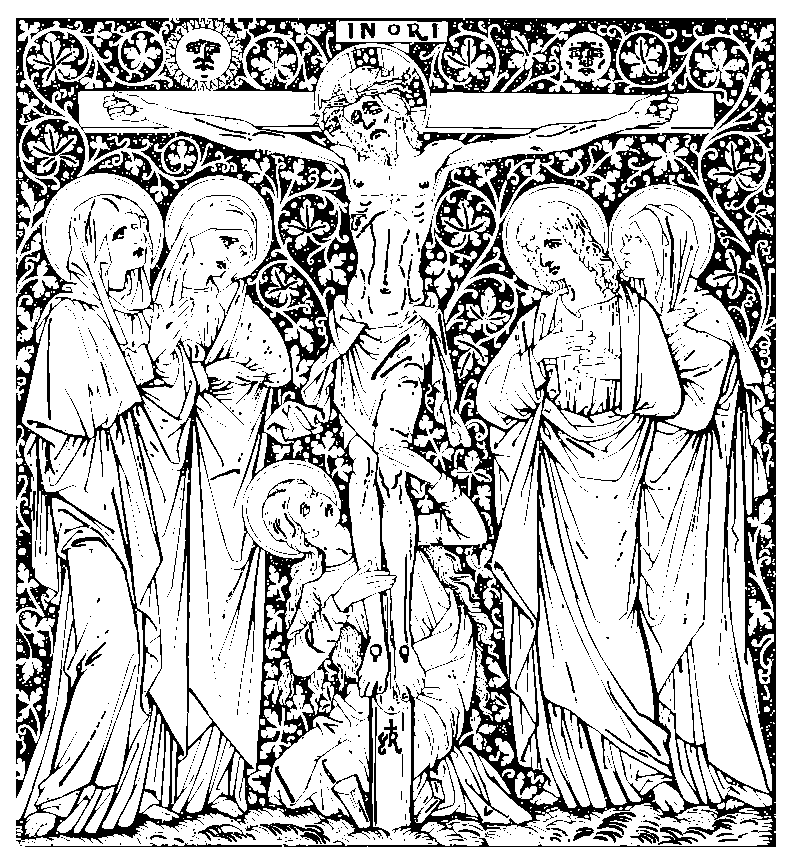
\includegraphics[width=1\textwidth,height=1\textheight,keepaspectratio]{media/pdf/ExaltationHolyCross}
\end{nscenter}

\begin{paracol}{2}\latim{
\rlettrine{E}{n} ego, o bone et dulcíssime Jesu, ante conspéctum tuum génibus me provólvo, ac máximo ánimi ardóre te oro atque obtéstor, ut meum in cor vívidos fídei, spei et caritátis sensus, atque veram peccatórum meórum pœniténtiam, eáque emmendándi firmíssimas voluntátem velis imprímere; dum magno ánimi afféctu et dolóre tua quinque vúlnera mecum ipse consídero ac mente contémplor, illud præ óculis habens, quod iam in ore ponébat tuo David prophéta de te, o bone Jesu: \emph{Ps. 21, 17-18} Fodérunt manus meas et pedes meos: dinumeravérunt ómnia ossa mea.
}\switchcolumn\portugues{
\rlettrine{E}{is-me} aqui, ó bom e dulcíssimo Jesus, de joelhos, ante a vossa divina presença, e Vos peço e suplico, com o mais ardente fervor da minha alma, que Vos digneis gravar no meu coração profundos sentimentos de fé, de esperança, de caridade, de verdadeiro arrependimento dos meus pecados e vontade firmíssima de me emendar, enquanto eu, com sincero afecto e intima dor de coração, considero e medito nas vossas Cinco Chagas, tendo bem presente aquelas palavras que o Profeta David já dizia de Vós, ó meu bom Jesus: \emph{Sl. 21, 17-18} «Traspassaram as minhas mãos e os meu pés, e contaram todos meus ossos».
}\end{paracol}

\subsubsection{Oblação de si próprio}

\begin{paracol}{2}\latim{
\rlettrine{S}{úscipe,} Dómine, univérsam meam libertátem. Accipe memóriam, intelléctum atque voluntátem omnem. Quidquid hábeo vel possídeo, mihi largítus es: id tibi totum restítuo, ac tuæ prorsus voluntáti trado gubernándum. Amórem tui solum cum grátia tua mihi dones, et dives sum satis, nec aliud quidquam ultra posco.
}\switchcolumn\portugues{
\rlettrine{A}{ceitai,} Senhor, em vossas mãos toda minha liberdade; recebei a minha memória, inteligência e vontade. Tudo o que tenho e possuo, fostes Vós, Senhor, quem mo destes: eu Vo-lo entrego, Senhor, sem reserva alguma, para que a vossa vontade de tudo disponha. Dai-me somente o vosso amor e a vossa graça e serei bastante rico: Vos não peço outra coisa.
}\end{paracol}

\subsubsection{Piedosa Oração}

\begin{paracol}{2}\latim{
\rlettrine{O}{bsécro} te, dulcíssime Dómine Jesu Christe, ut pássio tua sit mihi virtus, qua múniar, prótegar atque deféndar; vúlnera tua sint mihi cibus potúsque, quibus pascar, inébrier atque delécter; aspérsio Sánguinis tui sit mihi ablútio ómnium delictórum meórum; mors tua sit mihi vita indefíciens, Crux tua sit mihi glória sempitérna. In his sit mihi reféctio, exsultátio, sánitas et dulcédo cordis mei Qui vivis et regnas in sǽcula sæculórum. Amen.
}\switchcolumn\portugues{
\rlettrine{P}{ermiti,} ó meu dulcíssimo Jesus, eu Vos suplico, que a vossa Paixão seja para mim força que me guarde, proteja e defenda; que as vossas Chagas sejam para mim alimento e bebida que me sustentem, inebriem e alegrem; que a aspersão do vosso Sangue lave e apague todos meus pecados; que a vossa morte seja para mim vida sem fim; que a vossa Cruz seja para mim glória eterna; que tudo isto seja o meu alimento, a minha alegria, a minha saúde e a doçura do meu coração. Ó Vós, que viveis e reinais em todos os séculos dos séculos. Amen.
}\end{paracol}


\subsubsection{Oração à B. Virgem Maria}

\begin{paracol}{2}\latim{
\rlettrine{O}{} María, Virgo et Mater sanctíssima, ecce, suscépi dilectíssimum Fílium tuum, quem immaculáto útero tuo concepísti, genuísti, lactásti, atque suávissimis ampléxibus strinxísti. Ecce, cujus aspéctu lætabáris et ómnibus delíciis replebáris, illum ipsum tibi humíliter et amánter repræsénto et óffero tuis bráchiis constringéndum, tuo corde amándum, sanctissimǽque Trinitáti in suprémum latríæ cultum, pro tui ipsíus honóre et glória et pro meis totiúsque mundi necessitátibus, offeréndum. Rogo ergo te, piíssima Mater, ímpetra mihi véniam ómnium peccatórum meórum, uberémque grátiam ipsi deínceps fidélius serviéndi, ac deníque grátiam finálem, ut eum tecum laudáre possim per ómnia sǽcula sæculórum. Amen.
}\switchcolumn\portugues{
\slettrine{Ó}{} Maria, Virgem e Mãe santíssima, eis que acabo de receber no meu peito o vosso dilectíssimo Filho: Aquele mesmo que gerastes no vosso seio imaculado; destes à luz ao mundo; alimentastes; e tantas vezes apertastes em vossos amplexos castíssimos e amorosíssimos; Aquele mesmo cuja vista enchia a vossa alma de alegrias e de delícias! Eis que, cheio de humildade e de amor, eu vo-l’O entrego novamente em vossas mãos, para que O abraceis e entregueis à Santíssima Trindade, em culto supremo de latria, para honra e glória vossa e para alcançar as graças de que eu e o mundo temos necessidade. Eu vos suplico, ó piíssima Mãe, que me alcanceis o perdão de todos meus pecados e abundantes graças para Lhe obedecer fielmente, e, enfim, a graça da perseverança final, para que convosco possa louvá-l’O em todos os séculos dos séculos. Amen.
}\end{paracol}


\subsubsection{Oração a S. José}

\begin{paracol}{2}\latim{
\rlettrine{V}{írginum} custos et pater, sancte Joseph, cujus fidéli custódiæ ipsa Innocéntia Christus Jesus et Virgo vírginum María commíssa fuit: te per hoc utrúmque caríssimum pignus Jesum et Maríam óbsecro et obtéstor, ut me, ab omni immundítia præservátum, mente incontamináta, puro corde et casto córpore Jesu et Maríæ semper fácias castíssime famulári. Amen.
}\switchcolumn\portugues{
\slettrine{Ó}{} São José, pai e protector das almas virgens, guarda fiel a quem Deus confiou Jesus, a própria Inocência, e Maria, a Virgem entre as virgens, eu vos peço e suplico por Jesus e Maria, por este duplo depósito que Vos é tão querido, que me preserveis de qualquer impureza e disponhais que meu espírito seja isento de erros, o coração seja puro e o corpo casto, a fim de que sirva continuamente a Jesus e a Maria em perfeita castidade. Amen.
}\end{paracol}


\subsection{Oração ao Santo em cuja honra foi celebrada a Missa}

\begin{paracol}{2}\latim{
\rlettrine{S}{ancte} {\redx N.}, in cujus honórem incruéntum Córporis et Sánguinis Christi sacrifícium óbtuli, fac, tua poténti apud Deum intercessióne, ut, usu hujus mystérii, passiónis et mortis ejúsdem Christi Salvatóris nostri mérita cónsequar, ac, cum illíus frequentatióne, contínuo crescat meæ salútis efféctus Amen.
}\switchcolumn\portugues{
\rlettrine{S}{anto} {\redx N.}, em cuja honra celebrei (ou assisti ao) Sacrifício incruento do Corpo e do Sangue de Cristo, alcançai-me, com vossa intercessão junto de Deus, que, em virtude da celebração (ou participação) destes mistérios, os méritos da Paixão e da Morte do mesmo Cristo, nosso Salvador, sejam aplicadas em meu favor e que a frequente e contínua celebração (ou participação) destes mistérios me alcance os frutos da salvação. Amen.
}\end{paracol}
